\section{Introduction}
\label{sec:introduction}

% General introduction
PFunc, short for Parallel Functions, is a lightweight and portable library that
provides C and \Cpp{} APIs to express task parallelism. The features offered by
PFunc are a strict superset of the features offered by current solutions for
task parallelism.  Specifically, PFunc extends the feature set of current
solutions with custom task scheduling, task priorities and task affinities.
Furthermore, PFunc offers task groups for SPMD-style programming and multiple
task completion notifications for parallel execution of DAGs.  PFunc's extended
feature set is geared towards helping knowledgeable users optimize their
application performance. In this section, we describe PFunc with an emphasis on
its new features.  

% Explain the architecture
\subsection{Overview}
\label{sec:design}

\begin{figure}[t]
\centering
\includegraphics[width=0.6\textwidth]{figs/overview}
\caption{Internal organization of PFunc.}
\label{fig:overview}
\end{figure}

PFunc's design is based on the principles of generic and generative
programming. As a result, PFunc is able to offer a wide variety of
customizations to its users without incurring any runtime penalties.  Using
PFunc is a two step process. First, users generate a customized library
instance description that best suits their needs.  Second, the generated
library instance description is used to parallelize user applications.
Figure~\ref{fig:overview} provides a complete overview of the different 
components of PFunc. These are:

\begin{list}{\labelitemi}{\leftmargin=1em}
% Library instance
\item \textbf{Library instance:}
manages the threads and the task queues. The library instance can be thought of
as the ``runtime'' of PFunc.
% Tasks
\item \textbf{Tasks:}
are the units of parallelization in PFunc. Each task consists of a task handle,
a function (or function object) that is to be executed, task attributes that 
determine the execution parameters for the task and the group that this 
particular task belongs to.
\end{list}

Figure~\ref{fig:life_cycle} depicts the typical life-cycle of a PFunc
application.  First, the library is initialized. Then, tasks are spawned and
executed in parallel.  Finally, the library instance is cleared.

\begin{figure}[t]
\centering
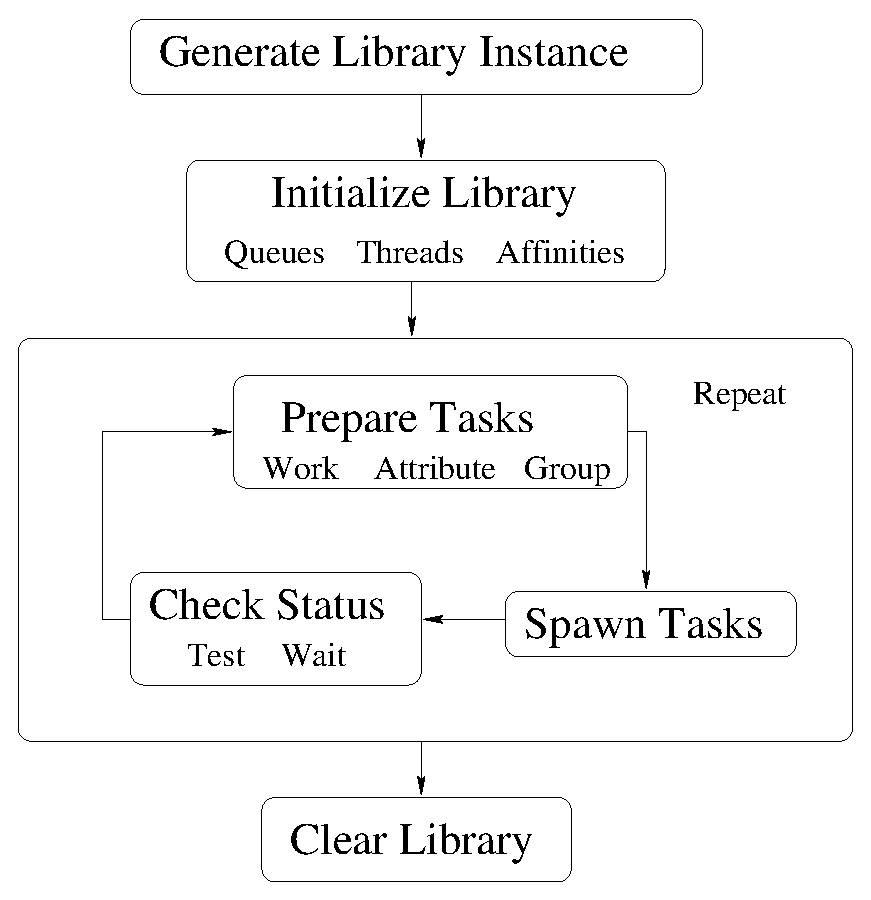
\includegraphics[width=0.5\textwidth]{figs/life-cycle}
\caption{Typical life-cycle of a PFunc application.}
\label{fig:life_cycle}
\end{figure}

The rest of this tutorial is organized as follows: Section~\ref{sec:generate}
shows how to generate a library instance description that best suits the user's
needs. Section~\ref{sec:initialize} shows the various parameters that can be
used for initialization. Section~\ref{sec:spawn} exposits on spawning tasks
using PFunc. Section~\ref{sec:fibonacci} builds a parallel version of the
recursive Fibonacci computation using PFunc. Section~\ref{sec:pack} describes 
utility functions that can be used for packing and unpacking function
parameters for PFunc's C interface.  Section~\ref{sec:attribute} explains the
use of task attributes in greater detail. Section~\ref{sec:group} explains the
use of task groups in greater detail.  Section~\ref{sec:exception} introduces
PFunc's exception handling mechanism.  Finally, Section~\ref{sec:perf}
introduces PFunc's performance profiling interface.
